\documentclass[10pt]{beamer}\usepackage[]{graphicx}\usepackage[]{color}
%% maxwidth is the original width if it is less than linewidth
%% otherwise use linewidth (to make sure the graphics do not exceed the margin)
\makeatletter
\def\maxwidth{ %
  \ifdim\Gin@nat@width>\linewidth
    \linewidth
  \else
    \Gin@nat@width
  \fi
}
\makeatother

\definecolor{fgcolor}{rgb}{0.345, 0.345, 0.345}
\newcommand{\hlnum}[1]{\textcolor[rgb]{0.686,0.059,0.569}{#1}}%
\newcommand{\hlstr}[1]{\textcolor[rgb]{0.192,0.494,0.8}{#1}}%
\newcommand{\hlcom}[1]{\textcolor[rgb]{0.678,0.584,0.686}{\textit{#1}}}%
\newcommand{\hlopt}[1]{\textcolor[rgb]{0,0,0}{#1}}%
\newcommand{\hlstd}[1]{\textcolor[rgb]{0.345,0.345,0.345}{#1}}%
\newcommand{\hlkwa}[1]{\textcolor[rgb]{0.161,0.373,0.58}{\textbf{#1}}}%
\newcommand{\hlkwb}[1]{\textcolor[rgb]{0.69,0.353,0.396}{#1}}%
\newcommand{\hlkwc}[1]{\textcolor[rgb]{0.333,0.667,0.333}{#1}}%
\newcommand{\hlkwd}[1]{\textcolor[rgb]{0.737,0.353,0.396}{\textbf{#1}}}%
\let\hlipl\hlkwb

\usepackage{framed}
\makeatletter
\newenvironment{kframe}{%
 \def\at@end@of@kframe{}%
 \ifinner\ifhmode%
  \def\at@end@of@kframe{\end{minipage}}%
  \begin{minipage}{\columnwidth}%
 \fi\fi%
 \def\FrameCommand##1{\hskip\@totalleftmargin \hskip-\fboxsep
 \colorbox{shadecolor}{##1}\hskip-\fboxsep
     % There is no \\@totalrightmargin, so:
     \hskip-\linewidth \hskip-\@totalleftmargin \hskip\columnwidth}%
 \MakeFramed {\advance\hsize-\width
   \@totalleftmargin\z@ \linewidth\hsize
   \@setminipage}}%
 {\par\unskip\endMakeFramed%
 \at@end@of@kframe}
\makeatother

\definecolor{shadecolor}{rgb}{.97, .97, .97}
\definecolor{messagecolor}{rgb}{0, 0, 0}
\definecolor{warningcolor}{rgb}{1, 0, 1}
\definecolor{errorcolor}{rgb}{1, 0, 0}
\newenvironment{knitrout}{}{} % an empty environment to be redefined in TeX

\usepackage{alltt}
% \usetheme{jhsph}
\usepackage[T1]{fontenc}
\setcounter{secnumdepth}{3}
\setcounter{tocdepth}{3}
\usepackage{url}
\usepackage{graphicx}
\ifx\hypersetup\undefined
  \AtBeginDocument{%
    \hypersetup{unicode=true,pdfusetitle,
 bookmarks=true,bookmarksnumbered=false,bookmarksopen=false,
 breaklinks=false,pdfborder={0 0 0},pdfborderstyle={},backref=false,colorlinks=false}
  }
\else
  \hypersetup{unicode=true,pdfusetitle,
 bookmarks=true,bookmarksnumbered=false,bookmarksopen=false,
 breaklinks=false,pdfborder={0 0 0},pdfborderstyle={},backref=false,colorlinks=false}
\fi
\usepackage{breakurl}

\makeatletter

%%%%%%%%%%%%%%%%%%%%%%%%%%%%%% Textclass specific LaTeX commands.
 % this default might be overridden by plain title style
 \newcommand\makebeamertitle{\frame{\maketitle}}%
 % (ERT) argument for the TOC
 \AtBeginDocument{%
   \let\origtableofcontents=\tableofcontents
   \def\tableofcontents{\@ifnextchar[{\origtableofcontents}{\gobbletableofcontents}}
   \def\gobbletableofcontents#1{\origtableofcontents}
 }


\usetheme{PaloAlto}

\makeatother
\IfFileExists{upquote.sty}{\usepackage{upquote}}{}
\begin{document}

\title[]{Accelerometry: Data structure and analysis}
\author[]{Andrew Leroux \& Jacek Urbanek \& Ciprian Crainiceanu}
\makebeamertitle





\section{Introduction}

\begin{frame}
\frametitle{NHANES accelerometry: Reproducing these Analyses}
\begin{itemize}
\item All analyses presented here can be replicated using the "CSS\_NHANES.R" script located at 
\url{https://www.github.com/andrew-leroux/CSS_NHANES/}
\item Steps:
    \begin{itemize}
    \item Download or clone
    \item Open R project ("CSS\_NHANES.Rproj")
    \item Open R script "CSS\_NHANES.R"
    \item Run code
    \end{itemize}
\end{itemize}
\end{frame}


\section{Background}


\begin{frame}
\frametitle{NHANES accelerometry}
\begin{itemize}
\item The National Health and Nutrition Survey is a cross-sectional study of the US population performed in 2-year waves
\item Complex survey structure (beyond the scope of this talk)
\item Accelerometry data available for the 2003-2004 and 2005-2006 waves
    \begin{itemize}
    \item Acceleration summarized into minute-level "activity counts"
    \item Up to 7 days of data for each participant
    \item Study protocol: remove the device at bedtime 
    \end{itemize}
\end{itemize}
\end{frame}



\begin{frame}
\frametitle{NHANES accelerometry: data structure}
\begin{itemize}
\item Accelerometry data downloadble from NHANES is in long format
\item Very large file sizes ($\approx$ 2.5 GB)
\item Unintuitive data structure
\end{itemize}
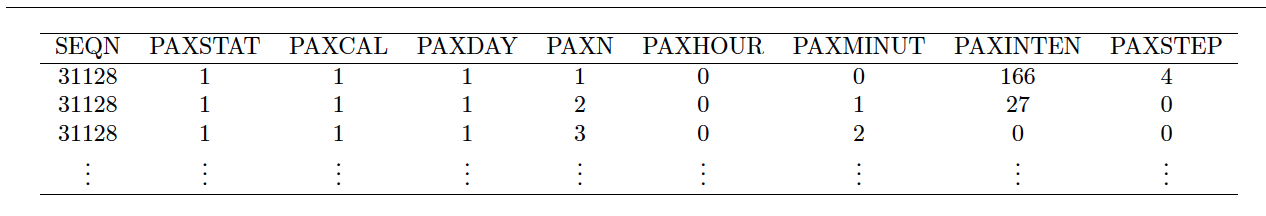
\includegraphics[width=\textwidth]{accel_data_long}
\end{frame}





\section{An NHANES data package}


\begin{frame}
\frametitle{NHANES accelerometry: proposed data strucutre}
\begin{itemize}
\item Wide format instead of long format\footnotemark ($\approx$ 60 MB)
\item 7 rows per participant, descending cronologoical order
\end{itemize}
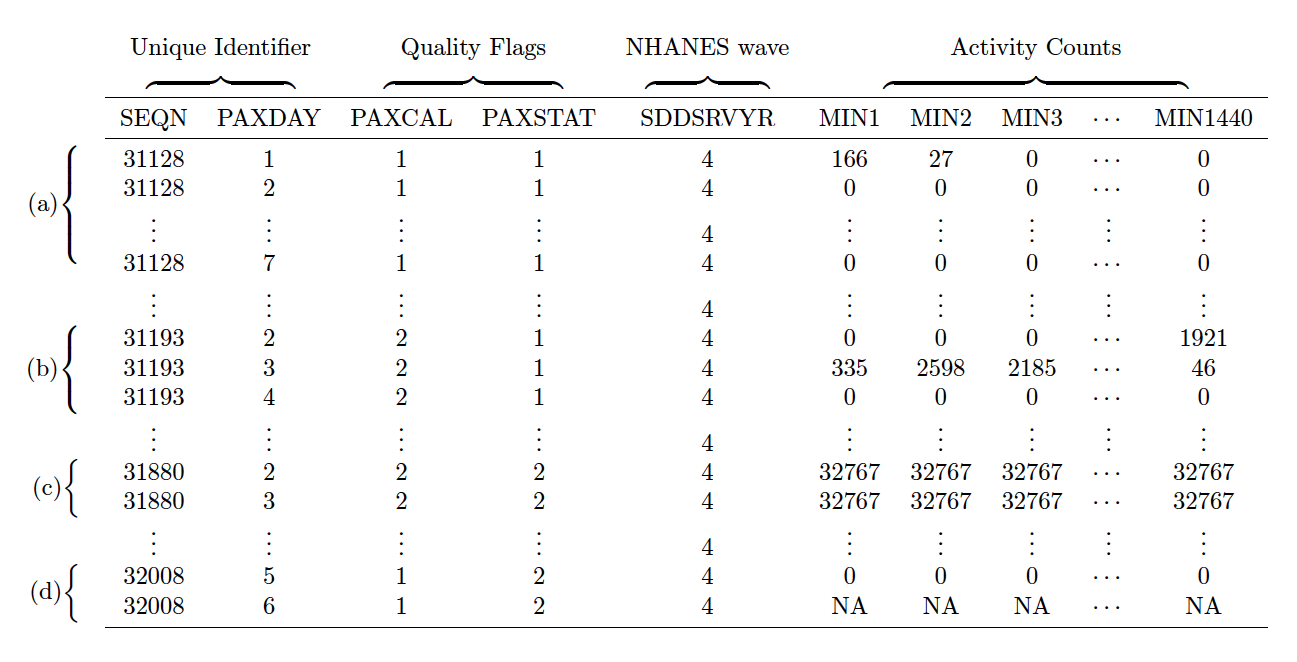
\includegraphics[width=\textwidth]{accel_data_wide}
\footnotetext{Leroux, A., Di, J., Smirnova, E. et al. Stat Biosci (2019). https://doi.org/10.1007/s12561-018-09229-9}
\end{frame}



\begin{frame}
\frametitle{NHANES accelerometry: {\it rnhanesdata} package}
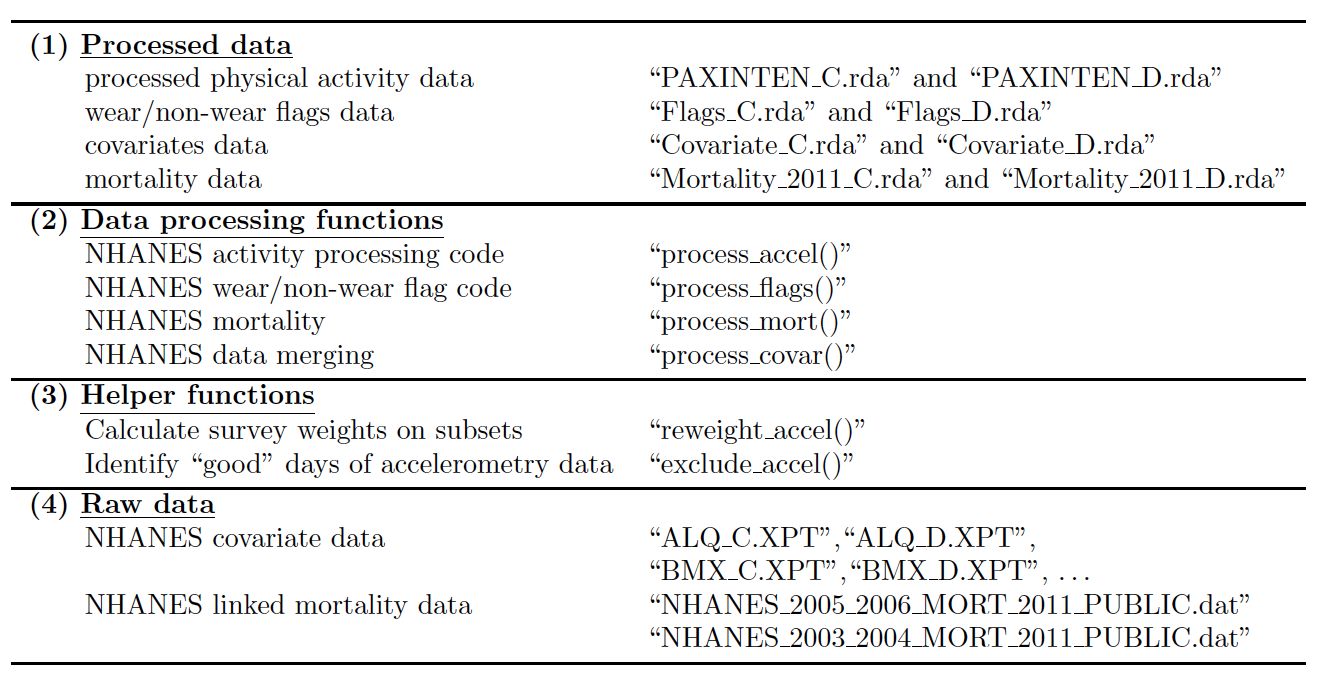
\includegraphics[width=\textwidth]{rnhanesdata}
\footnotetext{Leroux, A., Di, J., Smirnova, E. et al. Stat Biosci (2019). https://doi.org/10.1007/s12561-018-09229-9}
\end{frame}


\begin{frame}[fragile]
\frametitle{rnahnesdata: Package Installation}

\begin{itemize}
\item Package installation may take a few minutes due to the size of the processed data.
\item Requires the devtools package 
\item See ?"rnhanesdata-package" for details
\end{itemize}

\begin{knitrout}\small
\definecolor{shadecolor}{rgb}{0.969, 0.969, 0.969}\color{fgcolor}\begin{kframe}
\begin{alltt}
\hlkwa{if}\hlstd{(}\hlopt{!}\hlkwd{require}\hlstd{(}\hlstr{"rnhanesdata"}\hlstd{))\{}
    \hlstd{devtools}\hlopt{::}\hlkwd{install_github}\hlstd{(}\hlstr{"andrew-leroux/rnhanesdata"}\hlstd{)}
    \hlkwd{require}\hlstd{(}\hlstr{"rnhanesdata"}\hlstd{)}
\hlstd{\}}
\end{alltt}
\end{kframe}
\end{knitrout}
\end{frame}



\subsection{Data Analysis}


\begin{frame}
\frametitle{NHANES accelerometry: EDA}
\begin{itemize}
\item 7 days of data for two participants at the minute level
\item Estimated non-wear time has been imputed as 0
\item Dominated by a few very large values
\end{itemize}
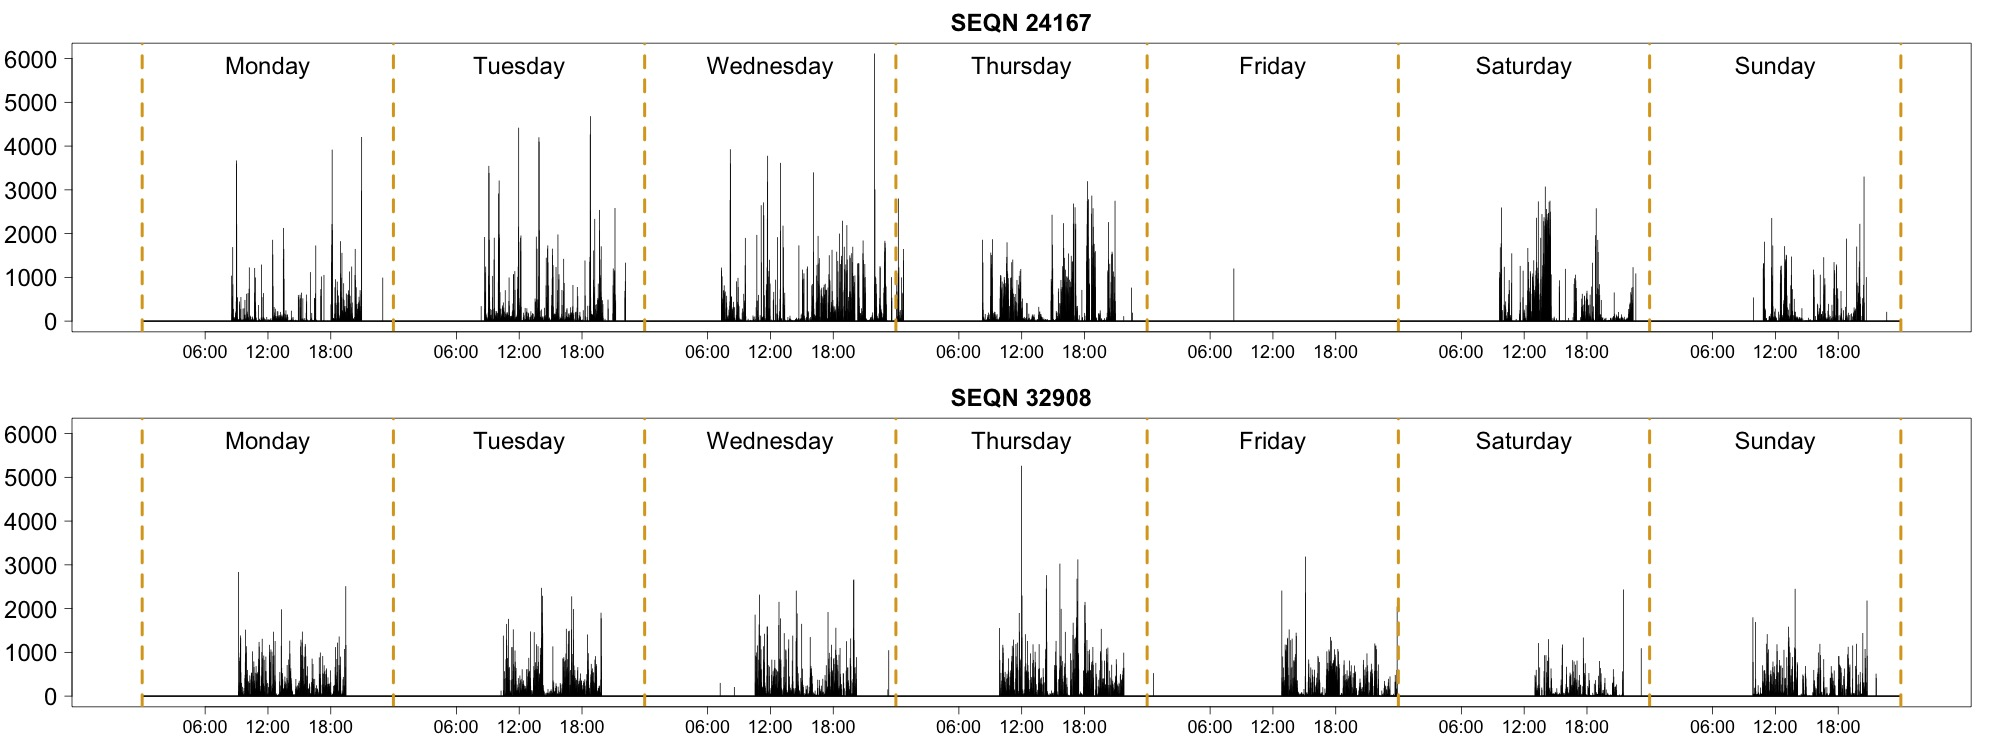
\includegraphics[width=\textwidth]{individual_profiles_raw}
\end{frame}

\begin{frame}
\begin{itemize}
\item Apply a $\log(1+x)$ transformaiton at the minute level
\item Still a high degree of minute-to-minute variability
\end{itemize}
\frametitle{NHANES accelerometry: EDA}
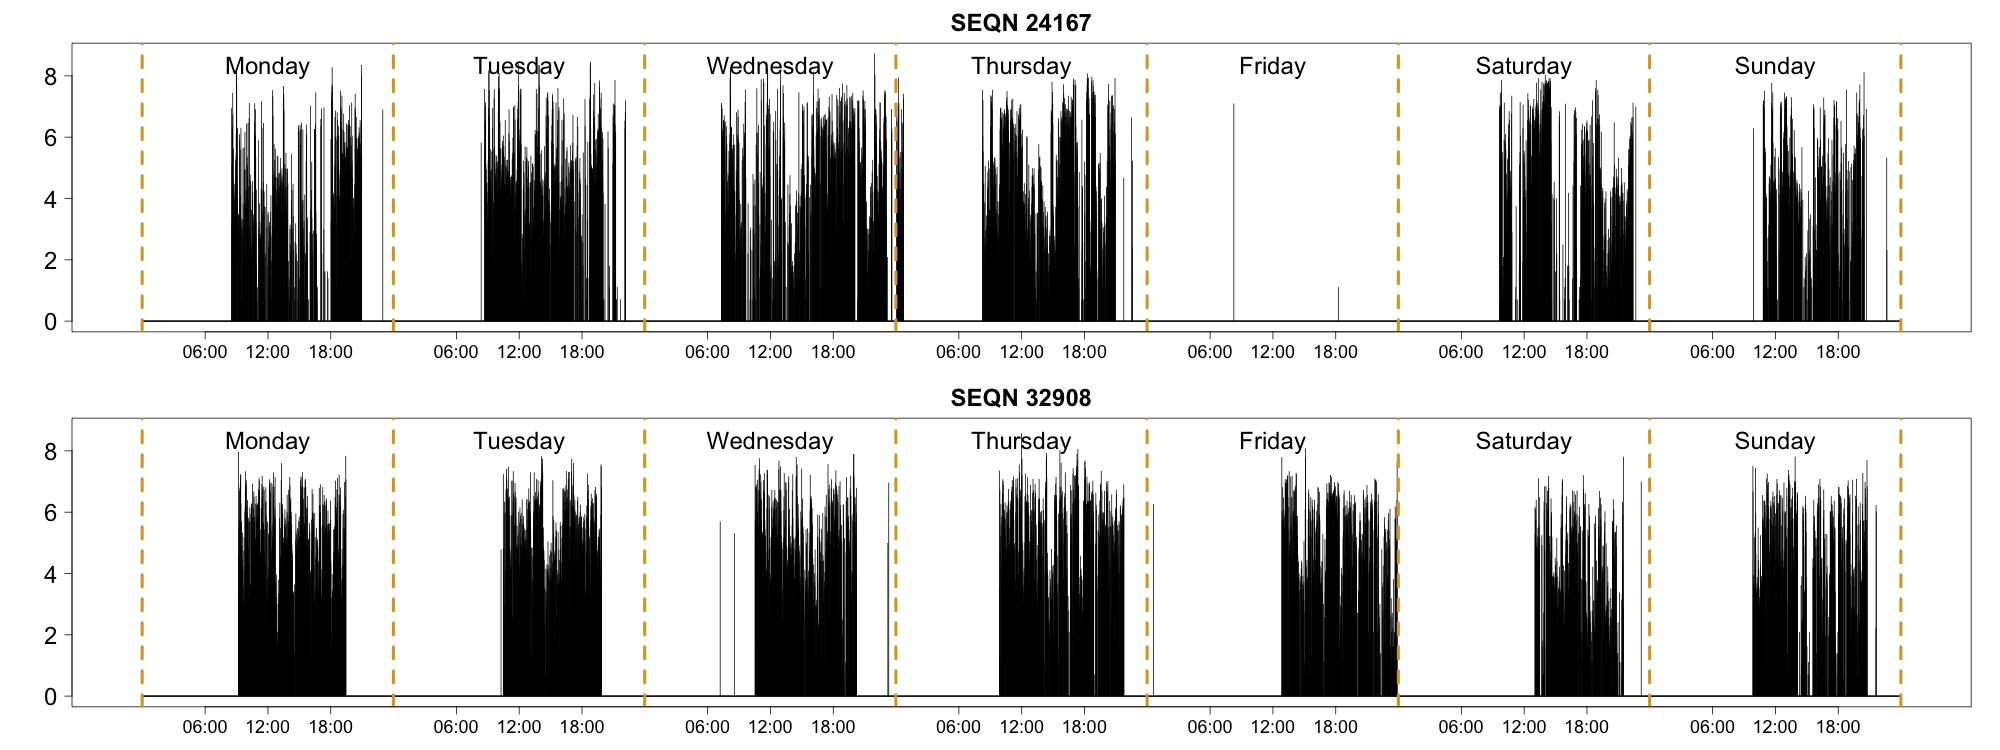
\includegraphics[width=\textwidth]{individual_profiles_trans}
\end{frame}


\begin{frame}
\begin{itemize}
\item Apply a $\log(1+x)$ transformaiton at the minute level
\item Still a high degree of minute-to-minute variability
\item Smooth the data
\end{itemize}
\frametitle{NHANES accelerometry: EDA}
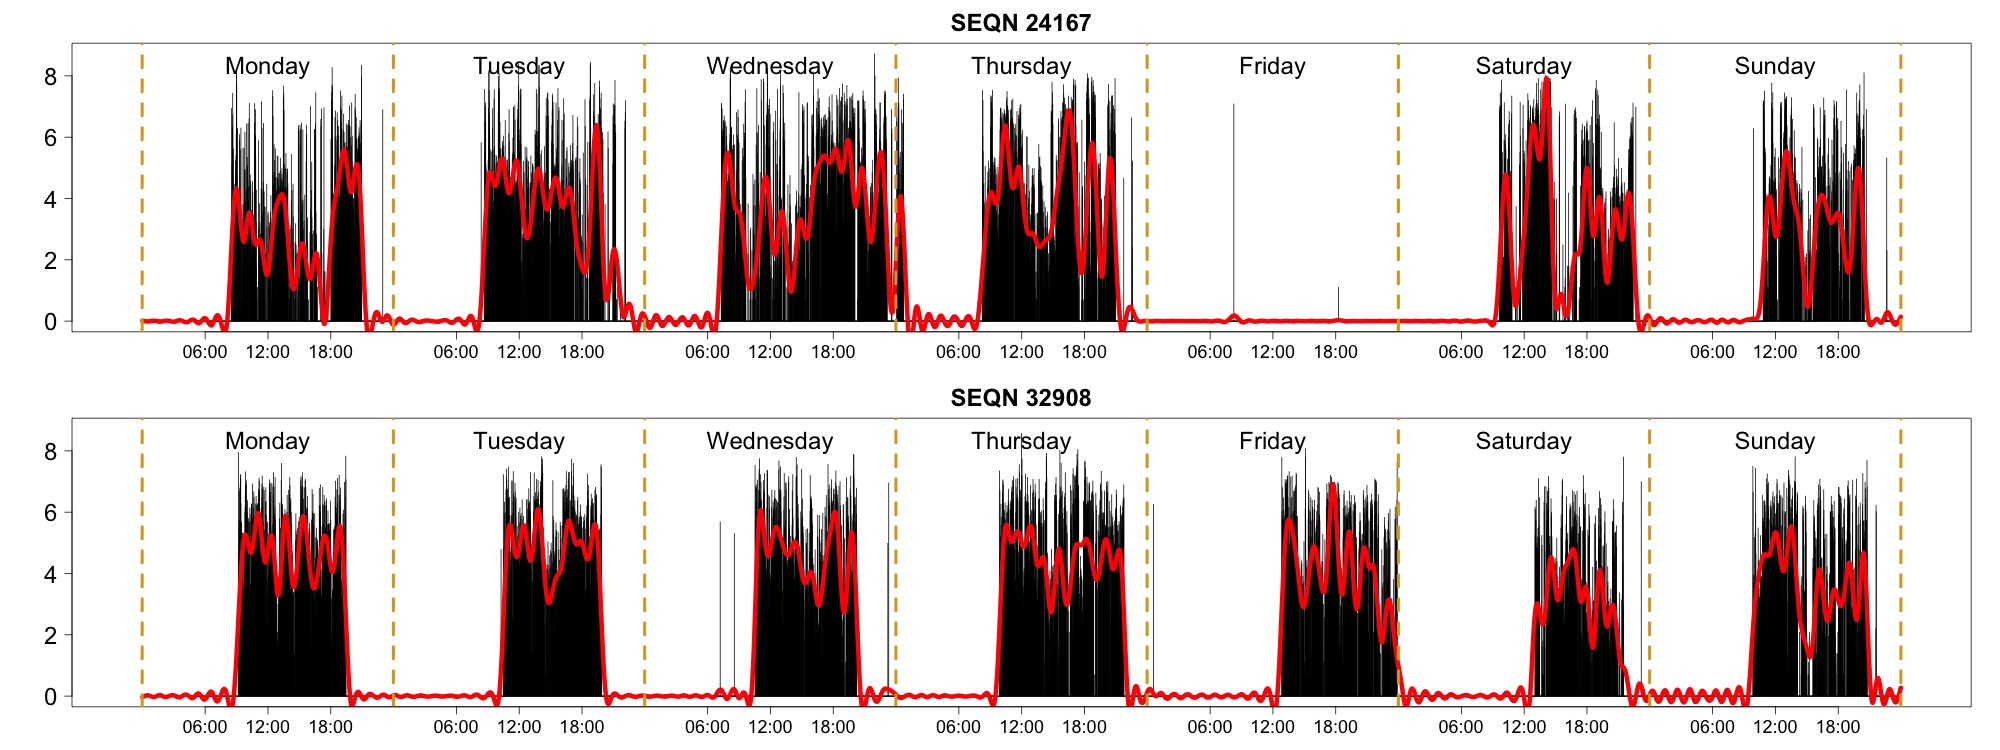
\includegraphics[width=\textwidth]{individual_profiles_trans_sm}
\end{frame}



\begin{frame}
\frametitle{NHANES accelerometry: EDA}
\begin{itemize} 
\item Visualizing the whole population
\item Subset based on $\geq 10$ hours of wear time, smooth the log transformed data, then average profiles across days within participants
\end{itemize}
\begin{center}
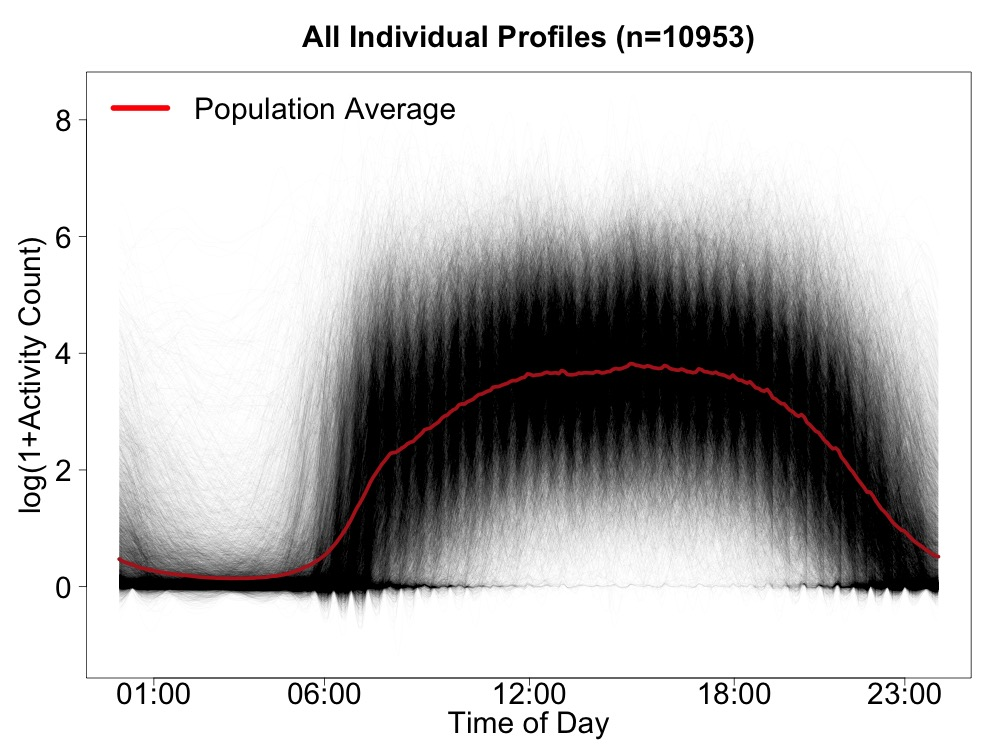
\includegraphics[width=0.75\textwidth]{population_curves}
\end{center}
\end{frame}



\begin{frame}
\frametitle{NHANES accelerometry: Analysis Procedure}
\begin{itemize}
\item Load and merge any relevant data by unique identifier (SEQN)
\item Apply exclusion criteria
    \begin{itemize}
    \item Data quality: 1) device calibration (PAXCAL); and 2) NHANES supplied flag (PAXSTAT)
    \item Adherence to wear-time protocol. Most studies use $\geq 10$ hours.
    \item Sufficient number of days of data. Most studies use $ \geq 3$ days of data with $\geq 10$ hours of wear.
    \item Other criteria: missing data, etc.
    \end{itemize}   
\item Apply binning or smoothing to the activity data if desired
\item Calculate features of interest
\item Incorporate survey design? Survey weights?
\item Regresison, machine learning, etc.
\end{itemize}
\end{frame}


\begin{frame}
\frametitle{NHANES accelerometry: Features}
\begin{itemize}
\item What even is an "activity count"?
\item Current standard: calculate single summaries of the data
    \begin{itemize}
    \item Volume of activity\footnotemark
        \begin{itemize}
        \item Time spent in sedentary/light/moderate/vigorous behaviours. Require population-specific studies to determine thresholds.
        \item Average daily total activity count (TAC). A proxy for total volume of moderate/vigorous activity
        \item Average daily total log activity count (TLAC). A proxy for total volume of low/light activity
        \end{itemize}
    \item Patterns of activity
        \begin{itemize}
        \item Fragmentation measures\footnotemark
        \item Timing of physical activity (activity profiles)
        \end{itemize}
    \end{itemize}
\item Here, we focuse on analyzing patterns of activity using subject-specific average activity profiles. 
\end{itemize}


\footnotetext{Varma VR, Dey D, Leroux A, et al. Total volume of physical activity: TAC, TLAC or TAC($\lambda$). Prev Med. 2017;106:233-235.}
\footnotetext{Di, J., Leroux, A., Urbanek, J., et al. Patterns of sedentary and active time accumulation are associated with mortality in US adults: The NHANES study. bioRxiv: 182337.}
\end{frame}





\begin{frame}
\frametitle{NHANES accelerometry: Analysis Procedure}
\begin{itemize}
\item In the subsequent analyses presented here we work with activity profiles
\item The data is smoothed, binned into 5 minute intervals, then averaged across days. 
This is done separately for the un-transformed and log-transformed activity counts
\item Binning is done mostly to reduce computational burden
\item None of the results here adjust for the survey design of NHANES 
\end{itemize}
\end{frame}












\section{Concluding Remarks}

\begin{frame}
\frametitle{Some Thoughts}
\begin{itemize}
\item D
\end{itemize}
\end{frame}



\begin{frame}
\frametitle{Open Problems}
\begin{itemize}
\item F
\end{itemize}
\end{frame}



\begin{frame}
\frametitle{In class exercises}
\begin{itemize}
\item Find 
\end{itemize}
\end{frame}





\end{document}
